% !TeX root = ../../thesis.tex
\chapter{From Perovskite Films to Photodetectors: Establishing a Baseline}\label{ch:material_properties}

The inception of the work presented in this thesis began with the repurposing an older vacuum evaporation chamber, previously used of the fabrication of organic thin film electronics. A significant portion of initial efforts focused on calibrating the chamber for the deposition of inorganic perovskite layers, evaluating film quality and repeatability, as well as investigating the effect of fundamental deposition parameters on the performance of the photodetector devices. In the first part of this chapter, we investigate the structural, optical, and crystallographic properties of co-evaporated \ch{CsPbI_2Br} thin films, as well as the effect of the post-deposition annealing step. In the second part of the chapter, we use the co-evaporated films to establish a baseline for photodetector device performance, considering factors like substrate type, transport layers, deposition rate, and stoichiometry. 

\section{Perovskite Deposition}

\begin{figure}
  \centering
  \medskip
  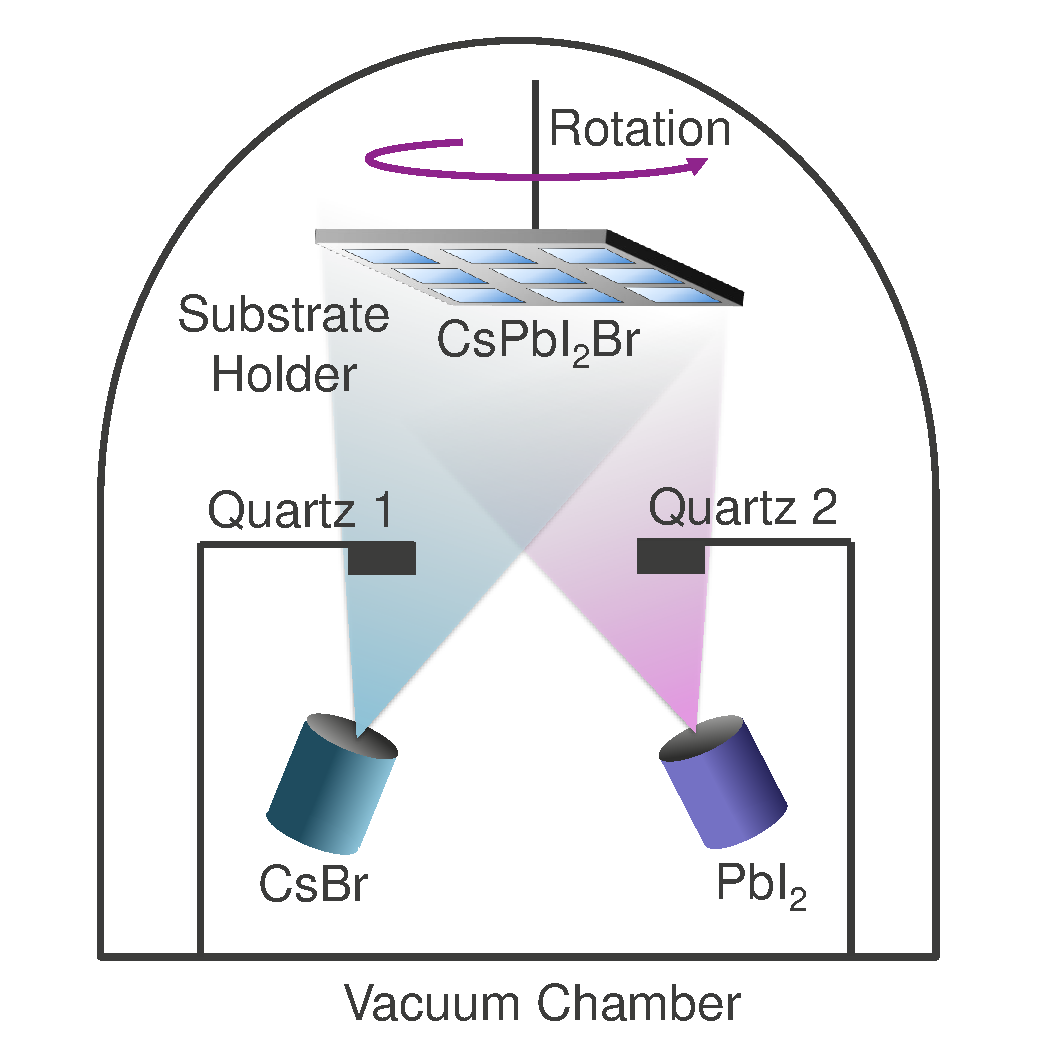
\includegraphics[width=.5\textwidth]{chapters/material_properties/images/Chamber.pdf}
  \caption[Short caption for Table of Figures]{Illustration of high-vacuum deposition chamber.}
  \label{fig:deposition_chamber}
\end{figure}




An illustration of the deposition chamber is provided in Figure~\ref{fig:deposition_chamber}. Two diametrically opposed sources are loaded with \ch{CsBr} and \ch{PbI_2} powders. Two separate quartz crystal microbalances (QCMs) are used to track the deposition rate of each source. The QCMs must be calibrated accordingly to the atomic mass of the precursor they are monitoring. To achieve this, an initial approximation of the tooling factor is made based on comparison with previous depositions. Subsequently, each precursor is deposited on \ch{Si/SiO_2} substrate, and the actual thickness is measured using spectroscopic ellipsometry or profilometry. The tooling factor is then adjusted using the equation: 

\begin{equation}
    TF_{\text{actual}} = TF_{\text{approx}} \times \frac{\text{thickness(actual)}}{\text{thickness(QCM)}}
\end{equation}

To account for system variability, we deposit each layer multiple times at different rates and target thicknesses. The final tooling factor of each source is calculated based on the average of all depositions.


Moving on to the co-evaporation of perovskite thin films, the ratio between the two sources' evaporation rates should be tuned to achieve the desired stoichiometry. For a stoichiometric film, the thickness ratio (TR) between two precursors, A and B, should be equal to: 

\begin{equation}
    TR = \frac{MolarMass(A)/Density(A)}{MolarMass(B)/Density(B)}.
\end{equation}

During the co-evaporation, a global shutter is protecting the samples while the sources are still heating up. Once both rates have reached their target value and are stabilized, the shutter is removed, initiating the deposition. The substrate holder, which can be loaded with 9 3$\times$3 $cm^2$ substrates, is kept at room temperature and rotates at 5 rounds per minute to ensure a uniform deposition. During the deposition, the temperature of each sources was continuously and automatically adjusted to maintain a constant evaporation rate. The deposition was automatically terminated once the target cumulative thickness was reached. For the development of the baseline evaporated films, a cumulative deposition rate of 0.8{\AA}/s and a \ch{CsBr:PbI_2} ratio of 1.05:1.00 was aimed for. Films were deposited with a slight excess of \ch{CsBr} since it was shown that it can improve the ambient stability of the black phase without compromising their optoelectronic properties \cite{Ma2017TheCells}. The nominal perovskite thickness was 275 nm. 

\subsection{Impact of Annealing on Material Properties}

The post-deposition annealing step of co-evaporated perovskite thin films is not strictly necessary, as the black phase can be achieved by properly tuning the deposition parameters---unlike sequentially evaporated films \cite{DongGrowthFilm}. However, thermal annealing does enhance the crystallinity of the films \cite{Frolova2017HighlyPbIsub2/sub}. 

\begin{figure}[htbp]
    \centering
    % First image (top)
    \begin{subfigure}[b]{\textwidth}
    \centering
        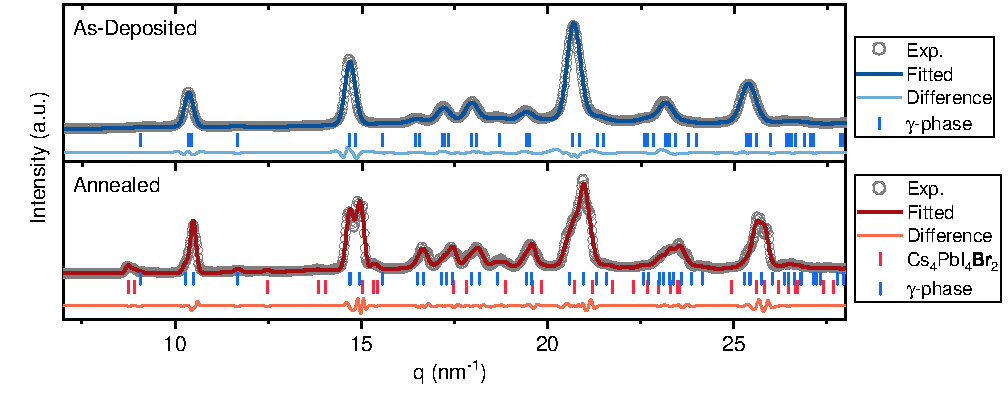
\includegraphics[width=0.85\linewidth]{chapters/material_properties/images/GIWAXS_Before_After.pdf}
        \caption{Caption for Image 1}
        \label{fig:ch2:giwaxs_before_after:model}
    \end{subfigure}

    \vspace{0.5cm}
    
    % Second image (bottom)
    \begin{subfigure}[b]{\textwidth}
    \centering
    \hspace{-1.4cm}
        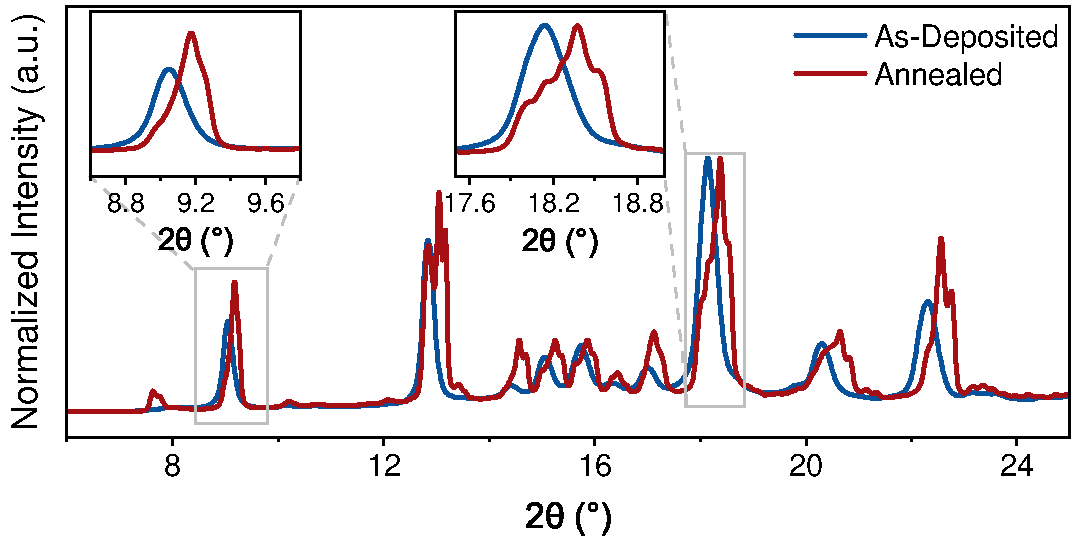
\includegraphics[width=0.68\linewidth]{chapters/material_properties/images/giwaxs_overlayed.pdf}
        \caption{Caption for Image 2}
        \label{fig:ch2:giwaxs_before_after:overlay}
    \end{subfigure}
    
    \caption{Overall caption for the figure.}
    \label{fig:ch2:giwaxs_before_after:}
\end{figure}


To investigate the effects of annealing on the properties of thermally evaporated \ch{CsPbI_2Br} thin films in detail, an as-deposited film (on a \ch{Si/SiO_2} substrate) was subjected to in-situ grazing incidence wide-angle X-ray scattering (GIWAXS). Specifically, while kept in a nitrogen environment, the sample was heated up to 300\degree C with a rate of 30\degree C/min. Once the target temperature was reached, the sample was allowed stabilize for 3 minutes before being cooled back down to room temperature at a similar rate. Fig.~\ref{fig:ch2:giwaxs_before_after:model} offers a comparison of the 1D integrated GIWAXS signals for the as-deposited and annealed perovskite states. All peaks in the diffraction pattern of the as-deposited state can be accounted for by the existence of a pure $\gamma$-\ch{CsPbI_2Br} phase, without indicating the presence any secondary phases, such as \ch{PbI_2}. This further highlights that the perovskite is formed in-situ onto the substrate. Achieving the in-situ black phase in co-evaporated \ch{CsPbI_3} thin films has previously been shown to require an elevated substrate temperature, around 50\degree C \cite{Dong2023GrowthFilm, Becker2019LowExperimentation}. The acquisition of the black perovskite phase at room temperature for our thermally evaporated films is attributed to the stabilizing effect of $Br^-$. 

The signal of the annealed perovskite state reveals the co-existence of the $\gamma$-\ch{CsPbI_2Br} phase and a 0D \ch{Cs_4PbX_6} phase, where X indicates the lattice's halogens. The main indicator for the emergence of the 0D phase is the peak that appears at 8.7 $nm^{-1}$. To further investigate the composition of the 0D phase we consider that both \ch{Cs_4PbI_6} and \ch{Cs_4PbBr_6} are stabilized in the same crystal structure (trigonal space group R-3c), which indicated that iodine and bromine can substitute for each other without altering the crystal geometry. Iodine has a larger ionic radius compared to bromine (2.2 {\AA} for $I^-$ compared to 1.96 {\AA} for $Br^-$), meaning that \ch{Cs_4PbI_6} would have larger lattice parameters than \ch{Cs_4PbBr_6} (a = b = 14.602 {\AA}, c = 18.268 {\AA} for the former, and a = b = 13.722 {\AA}, c = 17.299 {\AA} for the latter)\cite{Bhaumik2020BroadbandNanocrystals,DeBastiani2017InsideCrystals}. In our case, the lattice parameters are measured as a = b = 14.138 {\AA}, c = 17.828 {\AA}, clearly indicating that some of the iodine has been replaced by bromine.  Further analysis through Rietveld refinement, including occupancy refinement, confirms a stoichiometry of \ch{Cs_4PbI_4Br_2}. The 0D phase accounted for 10\% of the total perovskite volume, and its formation complicated the overall stoichiometry of the main phase. Its formation could potentially be attributed to the the excess of \ch{CsBr} during the co-evaporation process, however its amount is minimal and unlikely to affect the main phase's properties significantly \cite{Bai2019AStability}. 

More information about the structure of the annealed and as-deposited state can be extracted through Fig.~\ref{fig:ch2:giwaxs_before_after:overlay}, which provides an overlay comparison of the $2\theta$ GIWAXS signals. Through this comparison, three key changes can be observed (i) a reduction in the full width at half maximum (FWHM), (ii) peak shifting, and (iii) the appearance of peak asymmetry or splitting. The FWHM of the peaks is associated with crystallite size, as expressed through Scherrer's equation: 
 \begin{equation}
     D = \frac{k \times \lambda}{\beta \times cos\theta},
 \end{equation}

where k is the shape factor (0.9), $\lambda$ is the X-Ray wavelength, $\beta$ is the FWHM of the peak, and $\theta$ is the the Bragg peak position in radians. This calculation indicates that the crystallite size has nearly doubled as a result of the annealing process, increasing from 16 nm in the as-deposited state to 28 nm for the annealed one. In addition to the increase in crystallite size, the nonuniform peak shift towards right side and the appearance of peak asymmetry suggest that the annealing process has introduced macrostrain into the system. This strain could be attributed to two main factors: (i) the mismatch in the thermal expansion coefficients between the substrate and the thin film, which can induce biaxial strain at the interface \cite{Steele2019ThermalFilms}, and (ii) the coexistence of the 0D \ch{CsPbI_4Br_2} and the 3d \ch{CsPbI_2Br} phase, which may create lattice anchoring within the system \cite{Steele2022AnFilms, Saha2024Oxygen-MediatedPerformance}

\begin{figure}
  \centering
  \medskip
  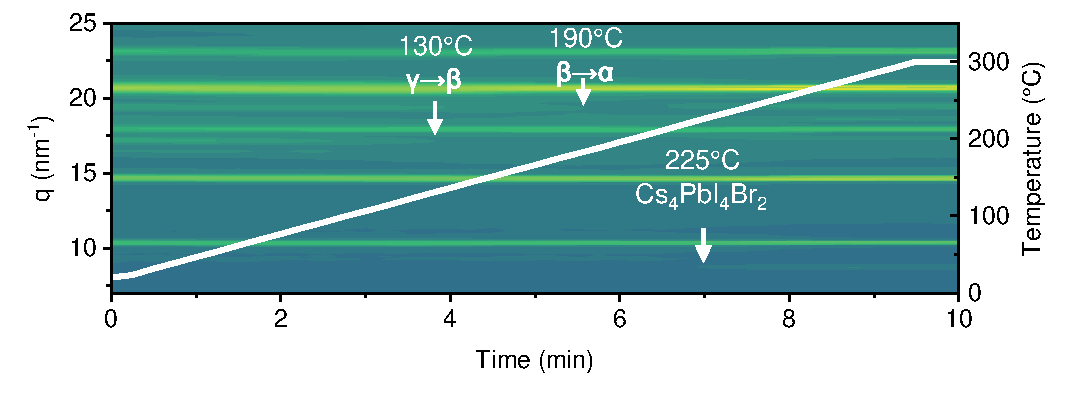
\includegraphics[width=\textwidth]{chapters/material_properties/images/GIWAXS_In_Situ.pdf}
  \caption[Short caption for Table of Figures]{In Situ GIWAXS}
  \label{fig:ch2:giwaxs_insitu}
\end{figure}

Fig.~\ref{fig:ch2:giwaxs_insitu} shows the in situ reduced 1D GIWAXS data during the temperature heating ramp. The transition from the orthorhombic ($\gamma$-) to the tetragonal ($\beta$-) phase is found to take place close to 130 \degree C, while the transition to the cubic ($a$-) phase happens at approximately 190 \degree C. Lastly, the emergence of the peak at 8.7 $nm^{-1}$ at 225 \degree C indicates the emergence of the 0D \ch{Cs_4PbI_4Br_2} phase. 


Fig.~\ref{fig:ch2:afm_sem} demonstrates the impact of this annealing step on the morphology of the perovskite film by comparing the AFM scan of the surface and the SEM image of the cross-section for the as-deposited and annealed state. The as-deposited state has grains of particularly small size, in the range of 30 - 40 nm (Fig.~\ref{fig:ch2:afm_before}), which is in agreement with previous reports on co-evaporated \ch{CsPbI_xBr_{3-x}} thin films \cite{Frolova2017HighlyPbIsub2/sub, Zhang2023SemitransparentAbsorber}. The RMS roughness is accordingly low and equal to 2 nm. Despite the small grain size, the cross-section of the film (Fig.~\ref{fig:ch2:sem_before}), shows a compact morphology without any noticeable defects, cracks or pinholes. The annealing step has a major effect on the morphology of the film, yielding a broad distribution of grain sizes, between 100 and 800 nm in diameter, as shown in the respective AFM image (Fig.~\ref{fig:ch2:afm_after}). The surface roughness has increased to 28.5 nm. At the same time, the SEM scan (Fig.~\ref{fig:ch2:sem_after}) reveals a grain-boundary-free cross-section, which is typically associated with improved optoelectronic properties. 

\begin{figure}[htbp]
    \centering
    % First row
    \begin{subfigure}[t]{0.45\textwidth}
        \centering
        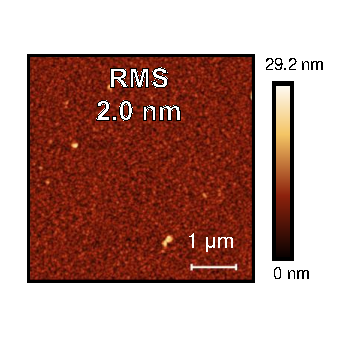
\includegraphics[width=\textwidth]{chapters/material_properties/images/AFM_before.pdf} 
        \caption{}
        \label{fig:ch2:afm_before}
    \end{subfigure}
    \hfill
    \begin{subfigure}[t]{0.45\textwidth}
        \centering
        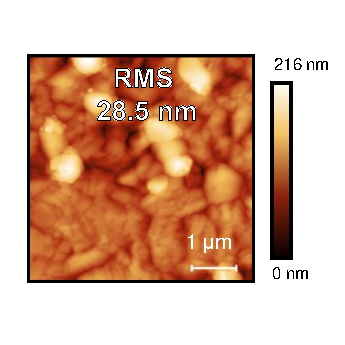
\includegraphics[width=\textwidth]{chapters/material_properties/images/AFM_after.pdf} % Replace with your image file        
        \caption{}
        \label{fig:ch2:afm_after}
    \end{subfigure}

    % Second row
    \begin{subfigure}[t]{0.4\textwidth}
        \centering
        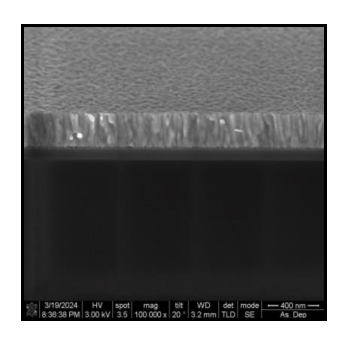
\includegraphics[width=\textwidth]{chapters/material_properties/images/SEM_Before.pdf} 
        \caption{}
        \label{fig:ch2:sem_before}
    \end{subfigure}
    \hfill
    \begin{subfigure}[t]{0.4\textwidth}
        \centering
        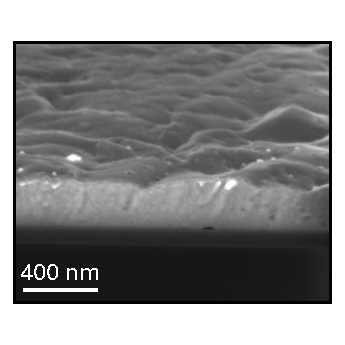
\includegraphics[width=\textwidth]{chapters/material_properties/images/SEM_After.pdf} 
        \caption{}
        \label{fig:ch2:sem_after}
    \end{subfigure}
    \caption{AFM and SEM images for the as-deposited and annealed perovskite sample.}
    \label{fig:ch2:afm_sem}
\end{figure}

\begin{figure}[htbp]
    \centering
    % First row
    \begin{subfigure}[t]{0.4\textwidth}
        \centering
        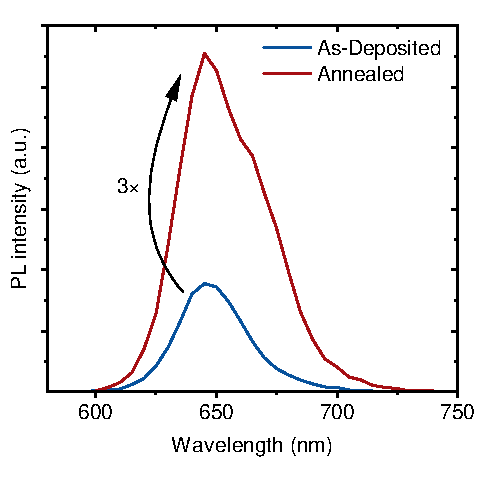
\includegraphics[width=\textwidth]{chapters/material_properties/images/SSPL.pdf} 
        \caption{}
        \label{fig:ch2:sspl}
    \end{subfigure}
    \hfill
    \begin{subfigure}[t]{0.4\textwidth}
        \centering
        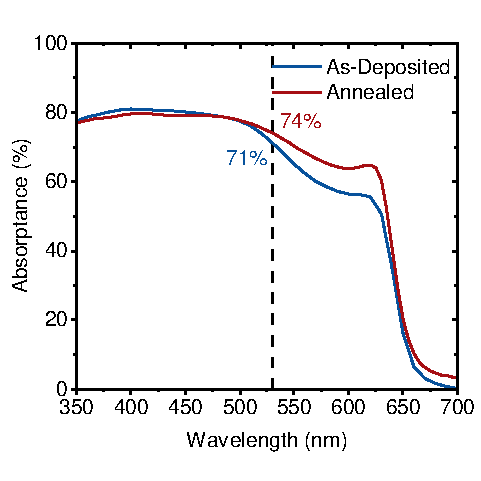
\includegraphics[width=\textwidth]{chapters/material_properties/images/Absorptance.pdf} % Replace with your image file
        \caption{}
        \label{fig:ch2:absorptance}
    \end{subfigure}

    \vspace{1em} % Space between rows

    % Second row
    \begin{subfigure}[t]{0.4\textwidth}
        \centering
        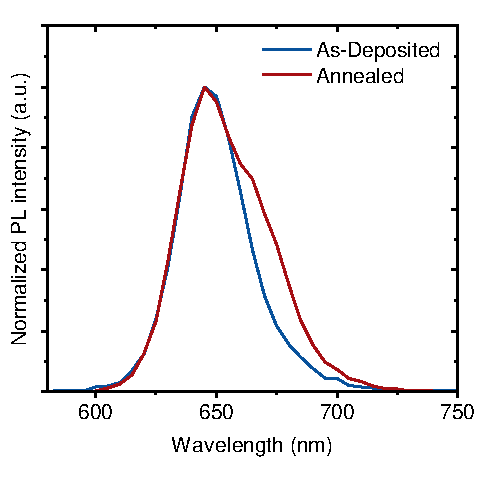
\includegraphics[width=\textwidth]{chapters/material_properties/images/SSPL_norm.pdf} % Replace with your image file
        \caption{}
        \label{fig:ch2:norm_sspl}
    \end{subfigure}
    \hfill
    \begin{subfigure}[t]{0.4\textwidth}
        \centering
        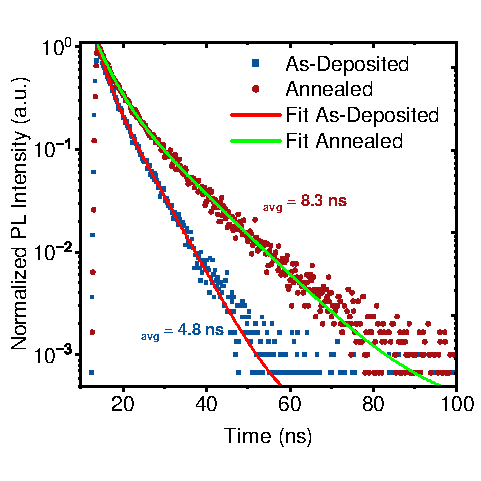
\includegraphics[width=\textwidth]{chapters/material_properties/images/TRPL_norm_double - Copy.pdf} % Replace with your image file
        \caption{}
        \label{fig:ch2:trpl}
    \end{subfigure}
    \caption{SSPL, TRPL, and absorptance for the an As-Deposited and an Annealed perovskite sample.}
\end{figure}



To further investigate the impact of the annealing step on the optoelectronic properties of the film, we deposit an identical perovskite film on a glass substrate and repeat the same annealing step, allowing as to perform steady and transient state photoluminescence (SSPL and TRPL), as well as absorptance measurements for the as-deposited and annealed perovskite state. The SSPL measurement in Fig.~\ref{fig:ch2:sspl}, indicates a 3-time increase in the intensity of the PL signal for the annealed film under a 530 nm excitation. This could potentially be attributed to increased absorptance at the excitation wavelength or a to a reduction of the non-radiative recombination pathways. The absorptance of the annealed film is indeed slightly higher at 530 nm, as demonstrated in Fig.~\ref{fig:ch2:absorptance}, however it is not sufficient to justify the increase in PL intensity. Therefore, the increase in crystallite size and the reduction of grain boundaries, as discussed above, contributed to minimizing non-radiative recombination mechanisms. It has to be noted, that there is no indication for the high-bandgap 0D \ch{Cs_4PbI_4Br_2} phase in the SSPL and absorptance spectra of the perovskite. This is in agreement with what was previously reported by Bai et al., who were able to detect the 0D phase in the absorptance spectrum only for highly non-stoichiometric films \cite{Bai2019AStability}. 

When comparing the normalized PL peaks for the as-deposited and annealed perovskite state, in Fig.~\ref{fig:ch2:norm_sspl}, an additional difference is observed, with the annealed film exhibiting a secondary, red-shifted shoulder inf its PL emission spectrum. This phenomenon was extensively studied by Schötz et al., and was attributed to a self-absorption of mechanism, whose impact is amplified by strong internal emissions and Urbach tail of the perovskite \cite{Schotz2020DoubleSelf-absorption}. As a resutlt, the increase in surface roughness that is introduced during the annealing of our thermally evaporated perovskite could explain the double peak emission via an increase in internal light scattering. Lastly, Fig.~\ref{fig:ch2:trpl} shows the TRPL spectra for the as-deposited and annealed perovskite state. A bi-exponential equation, described by the formula: 

\begin{equation}
    I_{PL}(t) = A_1exp(-\frac{t}{\tau_1}) + A_2exp(-\frac{t}{\tau_2}) + y_0,
\end{equation}

was able to accurately describe the decay of the both curves. Followingly, the average lifetime of the carriers was calculated using the equation: 
\begin{equation}
    \tau_{avg} = \frac{A_1 \tau_1^2 + A_2 \tau_2^2}{A_1 \tau_1 + A_2 \tau_2},
\end{equation}

indicating an almost doubling of the carriers' lifetime, from 4.8 ns for the as-deposited state to 8.3 ns for the annealed one.


\section{Device Development}

\begin{figure}[htbp]
    \centering
    % First plot
    \begin{subfigure}[t]{0.49\textwidth} % Adjust width as needed
        \centering
        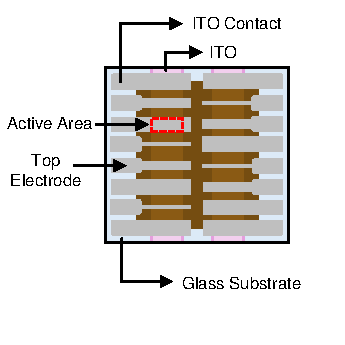
\includegraphics[width=\textwidth]{chapters/material_properties/images/Glass_Substrate.pdf} % Replace with your image
        \caption{}
        \label{fig:ch2:glass_substrate}
    \end{subfigure}
    \hfill % Space between the two plots
    % Second plot
    \begin{subfigure}[t]{0.49\textwidth} % Adjust width as needed
        \centering
        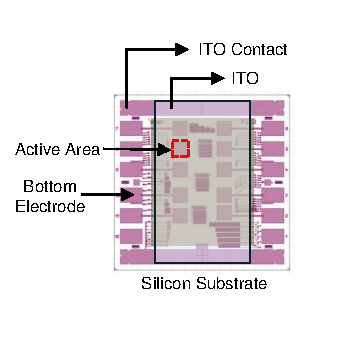
\includegraphics[width=\textwidth]{chapters/material_properties/images/PIX_Substrate.pdf} % Replace with your image
        \caption{}
        \label{fig:ch2:pix_substrate}
    \end{subfigure}

    % Caption for the whole figure
    \caption{Substrate layouts: (a) glass substrate, and (b) silicon substrate.}
    \label{fig:ch2:types_of_substrates}
\end{figure}


This section provides an overview of the parameters that can be varied during the development of perovskite-based photodetectors and their impact on device performance. As shown in Fig.\ref{fig:ch2:types_of_substrates}, two types of substrates were used in this study: glass substrates pre-patterned with an ITO contact (Fig.\ref{fig:ch2:glass_substrate}) and silicon substrates, designed internally and fabricated in imec's CMOS foundry, featuring a TiN bottom contact (Fig.~\ref{fig:ch2:pix_substrate}).

The fabrication process is similar for both substrate types, beginning with the deposition of the HTL (DC sputtered \ch{NiO_x}), followed by the deposition of the perovskite layer, the post-deposition annealing step, and finally, the deposition of the ETL. For glass substrates, the stack is completed by depositing Al contacts via thermal evaporation, using a shadow mask that defines 12 different devices. The device area is determined by the overlap between the ITO and Al electrodes, resulting in three different areas: 0.125 $cm^2$, 0.075 $cm^2$, and 0.025 $cm^2$. The use of variable-sized contacts allows for an analysis of the impact of device area on performance metrics.

For silicon substrates, the stack is completed with the deposition of an ITO sheet via linear magreton sputtering. In this case, the device area is defined by the bottom TiN contact, which is fixed at 0.0625 $cm^2$. The illumination setup differs between the two substrates: glass substrates are illuminated from the bottom (through the glass side - Fig.~\ref{fig:ch2:glass_stack}), while silicon substrates are illuminated from the top (through the ITO side - Fig.~\ref{fig:ch2:pix_stack}). 

The silicon substrates mimic the device structure used in the fabrication of imagers.2 However, due to their greater availability and accessibility, glass substrates are preferred for rapid prototyping and the screening of various deposition parameters and layers. Stacks that demonstrate promising performance are subsequently transferred and evaluated on silicon substrates. Despite the opposite orientation of the common contact, the results for both substrates are presented such that a negative bias consistently represents the reverse bias regime of the sample.


\begin{figure}[htbp]
    \centering
    % First plot
    \begin{subfigure}[t]{0.4\textwidth} % Adjust width as needed
        \centering
        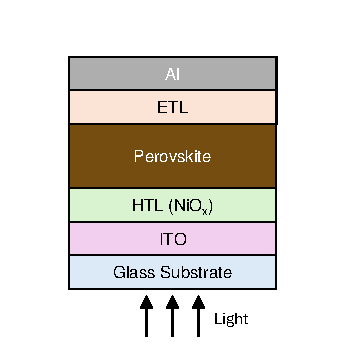
\includegraphics[width=\textwidth]{chapters/material_properties/images/Glass_Stack.pdf} % Replace with your image
        \caption{}
        \label{fig:ch2:glass_stack}
    \end{subfigure}
    \hfill % Space between the two plots
    % Second plot
    \begin{subfigure}[t]{0.4\textwidth} % Adjust width as needed
        \centering
        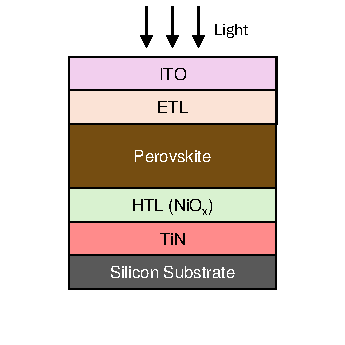
\includegraphics[width=\textwidth]{chapters/material_properties/images/PIX_Stack.pdf} % Replace with your image
        \caption{}
        \label{fig:ch2:pix_stack}
    \end{subfigure}

    % Caption for the whole figure
    \caption{Stack and illumination direction for (a) glass substrate, and (b) silicon substrate.}
    \label{fig:ch2:types_of_stacks}
\end{figure}

\subsection{Impact of Characterization Method and Statistical Remarks}

The characterization of the electrical performance of perovskite-based devices is not straight forward due to the presence of mobile ions in the lattice, which migrate under an applied and electric field, accumulate at the contacts and potentially participate in electrochemical reactions. In mixed-halide perovskites, phase segregation is another common occurrence. These are just some of the effects that occur under illumination or external bias, making it challenging to disentangle phenomena attributed to charge carriers, mobile ions, or newly formed species within the perovskite layer. A characteristic consequence of this complexity is hysteresis in J-V measurements, which has been shown to depend not only on the scan direction and speed, but also on the composition of the perovskite, the choice of transport layers, etc. 

\begin{figure}[htbp]
    \centering

    % First row
    \begin{subfigure}[b]{0.4\textwidth}
        \centering
        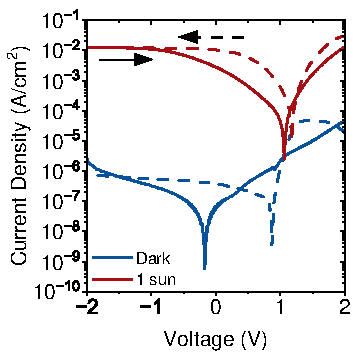
\includegraphics[width=\textwidth]{chapters/material_properties/images/Forward-Reverse-Plot.pdf}
        \caption{}
        \label{fig:ch2:scan_direction}
    \end{subfigure}
    \hfill
    \begin{subfigure}[b]{0.4\textwidth}
        \centering
        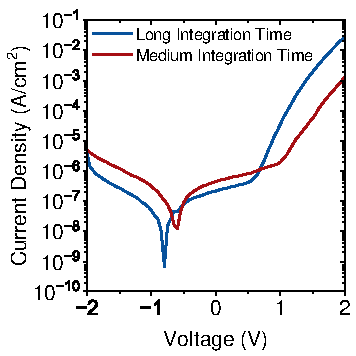
\includegraphics[width=\textwidth]{chapters/material_properties/images/Integration-Speed.pdf}
        \caption{}
        \label{fig:ch2:scan_speed}
    \end{subfigure}

    % Second row
    \begin{subfigure}[b]{0.35\textwidth}
        \centering        
        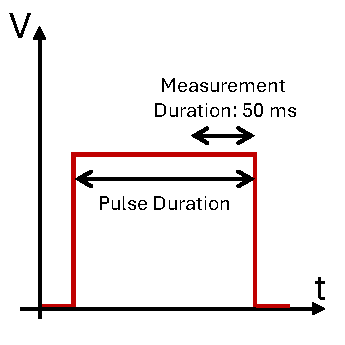
\includegraphics[width=\textwidth]{chapters/material_properties/images/PAIOS_Pulsed_Measurement.pdf}
        \caption{}
        \label{fig:ch2:pulsed_meas_PAIOS}
    \end{subfigure}
    \hfill
    \begin{subfigure}[b]{0.4\textwidth}
        \centering
        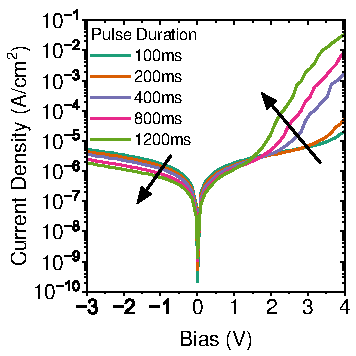
\includegraphics[width=\textwidth]{chapters/material_properties/images/Pulsed-PAIOS-plot.pdf}
        \caption{}
        \label{fig:ch2:pulsed_paios}
    \end{subfigure}


    % Third row - centered figure
    \begin{subfigure}[b]{0.4\textwidth}
        \centering
        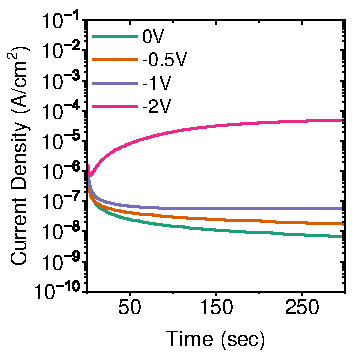
\includegraphics[width=\textwidth]{chapters/material_properties/images/Steady-State-plot.pdf}
        \caption{}
        \label{fig:ch2:steady_state}
    \end{subfigure}

    \caption{Impact of characterization methodology on device performance}
    \label{fig:ch2:types_of_measurement}
\end{figure}

Most commonly, the characterization of photodetectors relies on sequential J-V scans, which can be performed in dark and under illumination. Fig.~\ref{fig:ch2:scan_direction} shows the impact of the scan direction for one of the fabricated devices, while Fig.~\ref{fig:ch2:scan_speed} demonstrates the impact of the integration time. A significant hysteresis is observed, with the value of dark current, one of the most critical figures of merit of photodetectors, being highly dependent on the characterization settings. It is possible to eliminate hysteresis in the JV data by performing a pulsed IV measurement, the principle of which is demonstrated in Fig.~\ref{fig:ch2:pulsed_paios}. Specifically, each voltage step is applied as a pulse of specific length (pulse duration). The current value for each voltage step is the extracted as the average transient current during the specified measurement duration. This approach allows the ions to re-distribute for each voltage step, eliminating the hysteresis from the JV data (minimum $J_d$ is at 0 V, as shown in Fig.~\ref{fig:ch2:pulsed_meas_PAIOS}). However, even for this type of measurement, it is clear that the duration of each voltage pulse has a major impact on the measured J-V performance, with longer pulses leading to lower values of $J_d$ and larger values of forward current (rectification). (Why?) A last option for the characterization of the perovskite-based photodiodes is steady-state measurements, where a constant bias is applied and maintained for a prolonged period, until the value of monitored current starts saturating. This is demonstrated in Fig.~\ref{fig:ch2:steady_state}. A large drop in the value of $J_d$ is observed within the first seconds of the measurement, which was previously to depend on capacitive effects, rather than the presence of mobile ions \cite{Ollearo2021UltralowGeneration}. At -2 V, an almost 3-order increase in $j_d$ is observed, which has been associated with the breaking down of the device. This mechanism is concealed when performing J-V scans of relatively small duration and will be further investigate in Chapter~\ref{ch:transport_layer}. Considering the variability of results depending on the characterization approach, we mainly utilize sequential J-V scans, performed in the forward direction for comparing various stacks, stating that despite the impact of the measurement on the results, it still allows the fair identification of trends among different conditions. 


\begin{figure}[htbp]
    \centering
    % First plot
    \begin{subfigure}[t]{0.4\textwidth} % Adjust width as needed
        \centering
        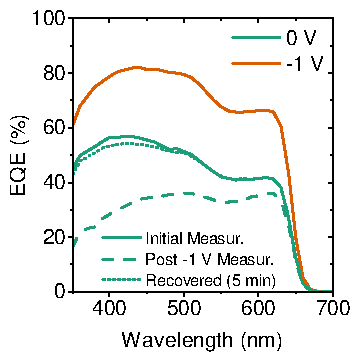
\includegraphics[width=\textwidth]{chapters/material_properties/images/EQE-1V.pdf} % Replace with your image
        \caption{}
        \label{fig:ch2:eqe-1V}
    \end{subfigure}
    \hfill % Space between the two plots
    % Second plot
    \begin{subfigure}[t]{0.4\textwidth} % Adjust width as needed
        \centering
        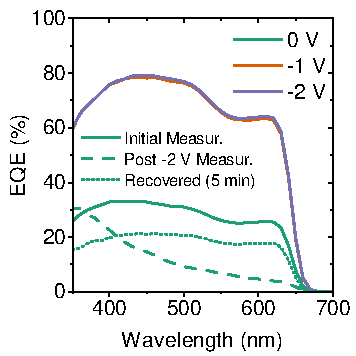
\includegraphics[width=\textwidth]{chapters/material_properties/images/EQE-2V.pdf} % Replace with your image
        \caption{}
        \label{fig:ch2:eqe-2V}
    \end{subfigure}

    
    \begin{subfigure}[t]{0.9\textwidth}
        \centering
        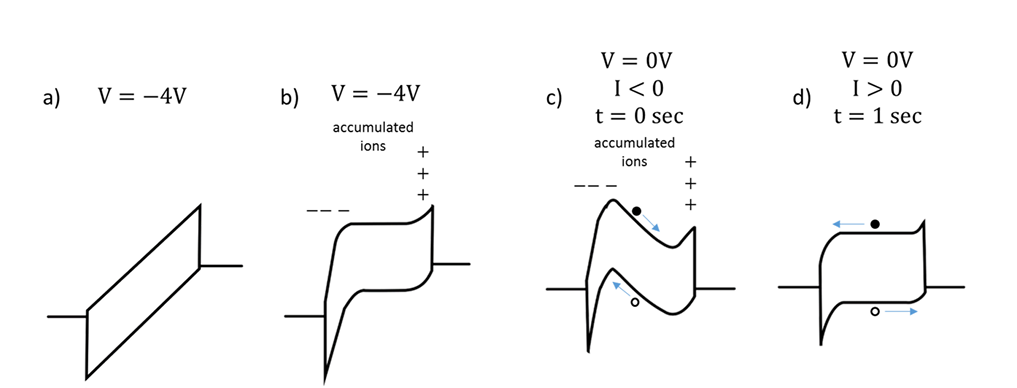
\includegraphics[width=\textwidth]{chapters/material_properties/images/ions.png} % Replace with your image file
        \caption{}
        \label{}
    \end{subfigure}

    % Caption for the whole figure
    \caption{Impact of measurement order on the EQE measurements.}
    \label{fig:ch2:eqe}
\end{figure}

The impact of the characterization approach on the acquired results extends to EQE measurements, as well. Fig.~\ref{fig:ch2:eqe-1V} and \ref{fig:ch2:eqe-2V} demonstrate the EQE results for two different devices that were fabricated on the same substrate. The EQE of the first device was measured sequentially at 0 V and -1 V, while the second device underwent measurements at 0 V, -1 V, and -2 V. Following these measurements, each device was subjected to two additional EQE measurements at 0 V: one immediately after the highest applied reverse bias (-1 V and -2 V, respectively) and another after a five-minute resting period in the dark. For both devices, the EQE at 0 V immediately after reverse biasing was significantly lower than the initial EQE measurement at 0 V. However, for the device biased up to -1 V, a five-minute resting period was sufficient to fully restore the initial EQE value. In contrast, for the device biased up to -2 V, the EQE at 0 V remained approximately 40\% lower than its initial value even after five minutes of recovery. This phenomenon could potentially be attributed to the accumulation of ions at the contacts and their potential contribution to electrochemical reactions, as demonstrated in Fig. xx. This experiment highlights the sensitivity of the acquired results to the prior biasing conditions. (Fing how much time it would take for the ions to re-distribute, and mention that is probably an electrochemical reaction that is taking place). From now on, the presented EQE results are performed on a new device, without prior bias, performed from the lowest to the highest reverse bias conditions. 

\begin{figure}[htbp]
    \centering
    % First row
    \begin{subfigure}[t]{0.4\textwidth}
        \centering
        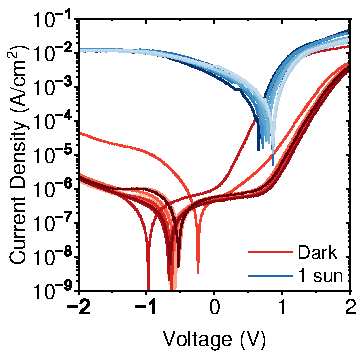
\includegraphics[width=\textwidth]{chapters/material_properties/images/High_yield_discrete.pdf} 
        \caption{}
        \label{fig:ch2:high_yield_discrete}
    \end{subfigure}
    \hfill
    \begin{subfigure}[t]{0.4\textwidth}
        \centering
        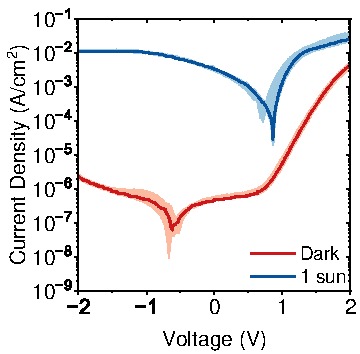
\includegraphics[width=\textwidth]{chapters/material_properties/images/High_yield_median.pdf} % Replace with your image file
        \caption{}
        \label{fig:ch2:high_yield_median}
    \end{subfigure}

    \vspace{1em} % Space between rows

    % Second row
    \begin{subfigure}[t]{0.4\textwidth}
        \centering
        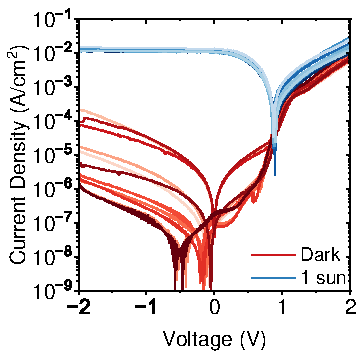
\includegraphics[width=\textwidth]{chapters/material_properties/images/low_yield_discrete.pdf} % Replace with your image file
        \caption{}
        \label{fig:ch2:low_yield_discrete}
    \end{subfigure}
    \hfill
    \begin{subfigure}[t]{0.4\textwidth}
        \centering
        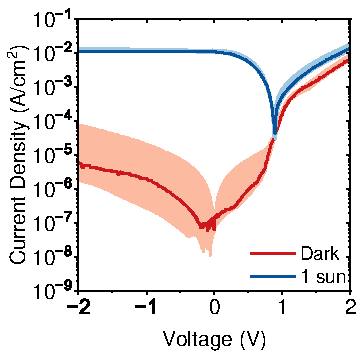
\includegraphics[width=\textwidth]{chapters/material_properties/images/low_yield_median.pdf} % Replace with your image file
        \caption{}
        \label{fig:ch2:low_yield_median}
    \end{subfigure}
    \caption{Discrete and statistical representation of J-V curves for samples with high and low variability.}
\end{figure}


Another important point is the related to the fair representation of the J-V data among the 12 devices on the same sample. Typically, there are a few outliers in each sample, the number of which defines the variability of a sample. This is more clearly illustrated in Fig.~\ref{fig:ch2:high_yield_discrete} and Fig.~\ref{fig:ch2:low_yield_discrete}, which represent two samples with small and large variability in device performance, respectively. In order to represent the median response of the sample, while also providing some insights into its variability we opt for presenting its performance in a statistical way, as shown in Fig.~\ref{fig:ch2:high_yield_median} and Fig.~\ref{fig:ch2:low_yield_median}, where the solid line represents the median response, while the shaded area represents the interquartile range. This way, the presence of 1 or 2 outliers in the device performance does not define the variability of the sample, which is reasonable considering the large area of the device and the likelihood of localized defects arising from process variations. 

Lastly, it is important to highlight the repeatability of device performance over different time periods. The fabrication tools used in this study were shared across multiple activities within the group, with occasional periods of downtime or non-standard behavior. Given the numerous variable parameters in a lab environment, pinpointing the exact causes of performance fluctuations is challenging. Inevitably, these variations also affected the performance of baseline devices. Consequently, the same device stack, when fabricated at different stages of the PhD work, may have exhibited varying degrees of performance fluctuation. This is noted to emphasize that, in this study, only samples fabricated within close temporal proximity are compared to identify trends and draw meaningful conclusions.

\subsection{Impact of Electron Transport Layer}

The first step in exploring device performance was selecting the transport layers for the PePD stack. The requirement for vacuum-deposited inorganic transport layers introduced several significant limitations. For the HTL, DC-sputtered \ch{NiO_x} was the only sufficiently mature option. However, due to the harsh conditions of the sputtering process, \ch{NiO_x} could only be deposited before the perovskite layer. For the ETL, the two most accessible candidates were e-beam deposited \ch{TiO_2} and thermally evaporated \ch{C_{60}}. Fig.~\ref{fig:ch2:tio2_compare} and Fig.~\ref{fig:ch2:c60_compare} compare the J-V scans of PePDs with \ch{TiO_2} and \ch{C_60} as the ETL, respectively. For each ETL, two versions of the stack were evaluated: one with an as-deposited perovskite layer and one with a flash-annealed perovskite layer. In the case of the annealed perovskite, annealing was performed before ETL deposition at 300 \degree C for 5–10 seconds in nitrogen environment. This was done considering that, while the as-deposited perovskite was already in the black phase, the annealed version exhibited higher crystallinity and improved optoelectronic properties, as discussed in the previous section.

\begin{figure}[htbp]
    \centering
    % First row
    \begin{subfigure}[t]{0.4\textwidth}
        \centering
        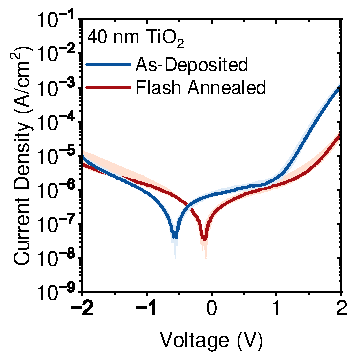
\includegraphics[width=\textwidth]{chapters/material_properties/images/TiO2-Compare.pdf} 
        \caption{}
        \label{fig:ch2:tio2_compare}
    \end{subfigure}
    \hfill
    \begin{subfigure}[t]{0.4\textwidth}
        \centering
        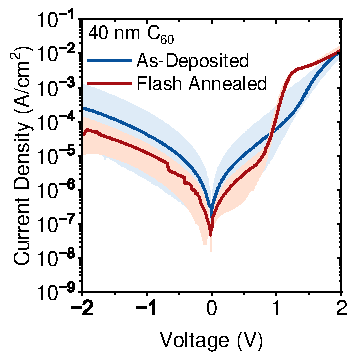
\includegraphics[width=\textwidth]{chapters/material_properties/images/C60-Compare.pdf} % Replace with your image file
        \caption{}
        \label{fig:ch2:c60_compare}
    \end{subfigure}


    % Second row
    \begin{subfigure}[t]{0.4\textwidth}
        \centering
        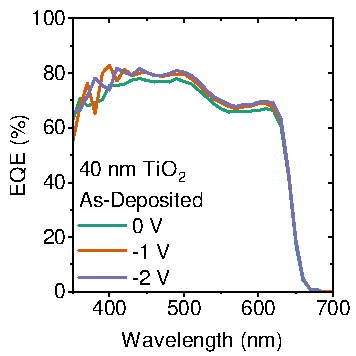
\includegraphics[width=\textwidth]{chapters/material_properties/images/As_Dep-EQE.pdf} % Replace with your image file
        \caption{}
        \label{fig:ch2:as_dep_eqe}
    \end{subfigure}
    \hfill
    \begin{subfigure}[t]{0.4\textwidth}
        \centering
        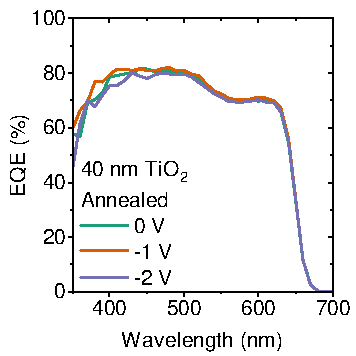
\includegraphics[width=\textwidth]{chapters/material_properties/images/Annealed_EQE.pdf} % Replace with your image file
        \caption{}
        \label{fig:ch2:annealed_eqe}
    \end{subfigure}
    \caption{Impact of transport layer and annealing conditions on device performance.}
\end{figure}

Both samples with \ch{TiO_2} exhibit similar levels of $J_d$ at -2 V, albeit the flash-annealed one has smaller hysteresis. The samples with \ch{C_60} exhibit significantly larger variability ans a median value of dark current at xx and yy for the as-deposited and annealed perovskite, respectively. Annealing the film seems to be reducing both the variability and the median value of dark current, however the performance is still superior compared to the samples with \ch{TiO_2}. It was previously shown that evaporated \ch{C_60} has the tendency to diffuse through the grain boundaries of the perovskite film, leading to potential shunts, and that is why it is mitigated with the annealing and larger grains. This phenomenon will be further investigated in Section xx. For this reason, for now we rely on the use of \ch{TiO_2} for the development of the baseline device stack. 

In terms of EQE for the \ch{TiO_2} samples, both exhibit a very similar behavior with an EQE that is already saturated at 0 V and is mainly above 70\% for the whole visible spectrum. These results further highlight the possibility of fabricating photodetectors processed solely at room temperature, a property that could open up new pathways for use with flexible substrates. However, considering the improvements in crystallinity and reduction in non-radiative recombination that were established for the annealed state, we move forward using the the flash-annealed sample with 40 nm of \ch{TiO_2} as the baseline. 


\subsection{Impact of Perovskite Deposition Conditions}

Beside the choice of transport layer and annealing of the perovskite, we wanted to explore the composition of the perovskite film, as well as the deposition speed on the performance. In terms of deposition rate we explore three deposition rates, ranging between 0.8, 1.2, and 1.6 {\AA}/sec. The overall performance is not drastically affected, however careful consideration of the $J_d$ at -2 V demonstrates an increase in the median value with faster deposition rate. Therefore, we maintain a deposition rate of 0.8 {\AA}/s for the rest of our experiments. 

In terms of stoichiometry, we vary the \ch{CsBr}:\ch{PbI_2} ratio between 0.8:1.0 (\ch{PbI_2} excess), 1.05:1.0 (Stoich), and 1.2:1.0 (\ch{CsBr} excess). For the samples with excess of \ch{PbI_2}, a significant overshoot is observed at the TPC measurement, typically associated with the accumulation of trapped charges at the interface, that limit the extraction of photo-generated carriers. Say something about sample with excess of CsBr...


\begin{figure}[htbp]
    \centering
    % First row
    \begin{subfigure}[t]{0.4\textwidth}
        \centering
        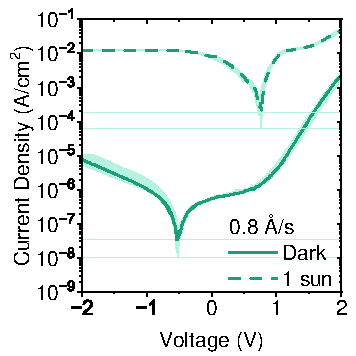
\includegraphics[width=\textwidth]{chapters/material_properties/images/08As-JV.pdf} 
        \caption{}
        \label{fig:ch2:0.8A/s-jv}
    \end{subfigure}
    \hfill
    \begin{subfigure}[t]{0.4\textwidth}
        \centering
        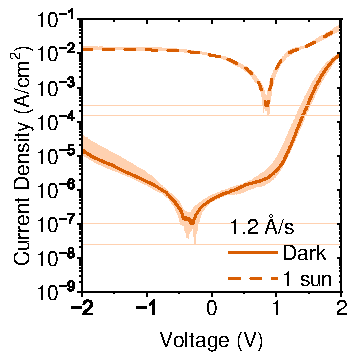
\includegraphics[width=\textwidth]{chapters/material_properties/images/12AS-JV.pdf} % Replace with your image file
        \caption{}
        \label{fig:ch2:1.2A/s-vj}
    \end{subfigure}

    % Second row
    \begin{subfigure}[t]{0.4\textwidth}
        \centering
        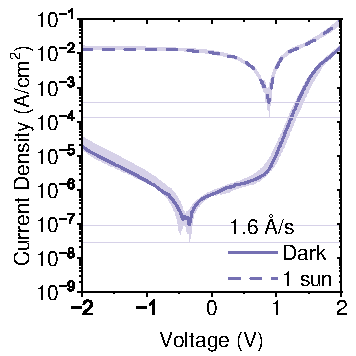
\includegraphics[width=\textwidth]{chapters/material_properties/images/16AS-JV.pdf} % Replace with your image file
        \caption{}
        \label{fig:ch2:1.6A/s-jv}
    \end{subfigure}
    \hfill
    \begin{subfigure}[t]{0.4\textwidth}
        \centering
        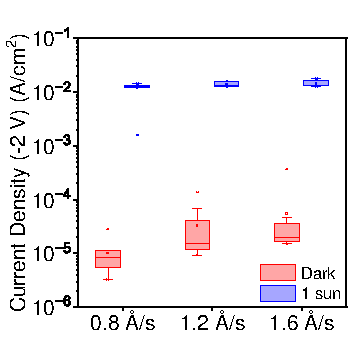
\includegraphics[width=\textwidth]{chapters/material_properties/images/Evap_Rate_Box_Plot.pdf} % Replace with your image file
        \caption{}
        \label{fig:ch2:box_plot_evap_rate}
    \end{subfigure}
    \caption{SSPL, TRPL, and absorptance for the an As-Deposited and an Annealed perovskite sample.}
\end{figure}




\begin{figure}[htbp]
    \centering

    % First row
    \begin{subfigure}[b]{0.3\textwidth}
        \centering
        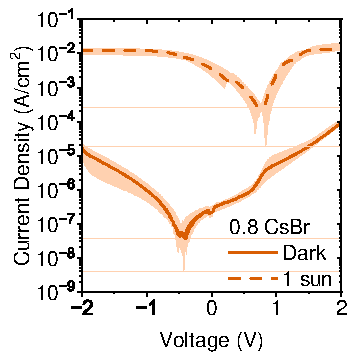
\includegraphics[width=\textwidth]{chapters/material_properties/images/08CsBr.pdf}
        \caption{}
    \end{subfigure}
    \hfill
    \begin{subfigure}[b]{0.3\textwidth}
        \centering
        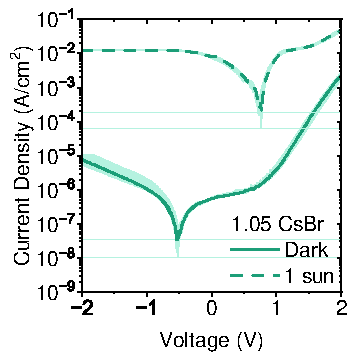
\includegraphics[width=\textwidth]{chapters/material_properties/images/105CsBr.pdf}
        \caption{}
    \end{subfigure}
    \hfill
    \begin{subfigure}[b]{0.3\textwidth}
        \centering
        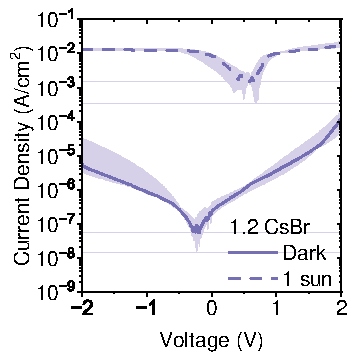
\includegraphics[width=\textwidth]{chapters/material_properties/images/12CsBr.pdf}
        \caption{}
    \end{subfigure}

    \vspace{1em} % Space between rows

    % Second row
    \begin{subfigure}[b]{0.28\textwidth}
        \centering
        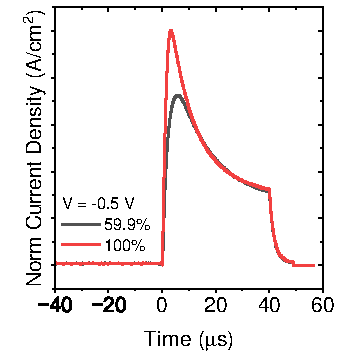
\includegraphics[width=\textwidth]{chapters/material_properties/images/TPC-08CsBr.pdf}
        \caption{}
    \end{subfigure}
    \hfill
    \begin{subfigure}[b]{0.28\textwidth}
        \centering
        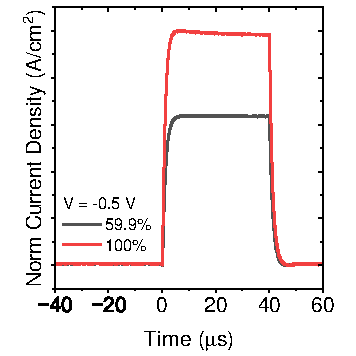
\includegraphics[width=\textwidth]{chapters/material_properties/images/TPC-105CsBr.pdf}
        \caption{}
    \end{subfigure}
    \hfill
    \begin{subfigure}[b]{0.28\textwidth}
        \centering
        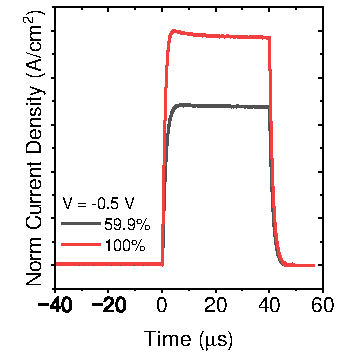
\includegraphics[width=\textwidth]{chapters/material_properties/images/tpc-12CsBr.pdf}
        \caption{}
    \end{subfigure}

    \caption{A figure with 2 rows and 3 images in each row.}
    \label{fig:two_rows_three_columns}
\end{figure}

\subsection{Impact of Substrate}

So far, we have established as the baseline stack the one deposited with a total deposition rate of 0.8{\AA}/s, at a stoichiometry of 1.05:1.00 CsBr:\ch{PbI_2}, with 40 nm of \ch{TiO_2} as the ETL. At this point we can transfer the same stack to the silicon substrates (Fig.~\ref{fig:ch2:pix_stack}). 
The device on silicon substrate exhibits significantly higher hysteresis and lower rectification, mainly attributed to the higher resistance of the TiN contact. In terms of the device's EQE, a significantly lower response at 0 V compared to the glass substrate. When increasing the bias to -1 V, it is possible to saturate, again. The slow turn-on of the diode is more explicitly illustrated at the EQE as a function of bias. 



\begin{figure}[htbp]
    \centering
    \begin{subfigure}{0.32\textwidth}
        \centering
        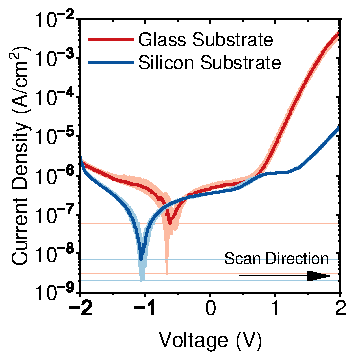
\includegraphics[width=\textwidth]{chapters/material_properties/images/JV_PIX_Glass.pdf}
        \caption{}
        \label{fig:ch2:jv_comp_pic_glass}
    \end{subfigure}
    \hfill
    \begin{subfigure}{0.32\textwidth}
        \centering
        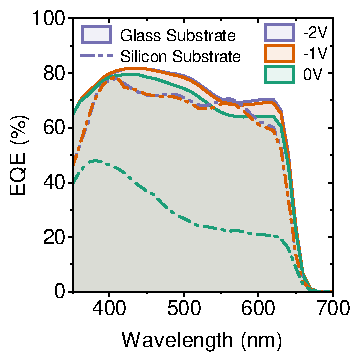
\includegraphics[width=\textwidth]{chapters/material_properties/images/EQE_fnm_PIX_Glass.pdf}
        \caption{}
        \label{fig:ch2:eqe_comp_pix_glass}
    \end{subfigure}
    \hfill
    \begin{subfigure}{0.32\textwidth}
        \centering
        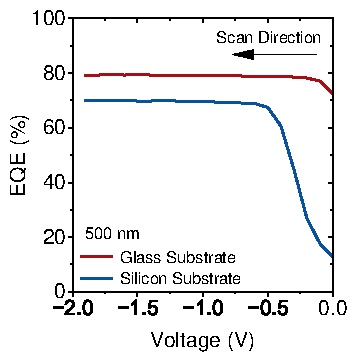
\includegraphics[width=\textwidth]{chapters/material_properties/images/EQE_fV_PIX_Glass.pdf}
        \caption{}
        \label{fig:plot3}
    \end{subfigure}
    
    \caption{A 1×3 grid of images.}
    \label{fig:ch2:eqefV_comp_pix_glass}
\end{figure}


Two potential causes could be evaluated for the slower turn-on of the diode when it is fabricated on top of the Si substrate. In contrast to ITO and Al that were used as contacts for the glass substrate, which have a large difference in the work function, ITO and TiN do not have a big difference in their work function. To further evaluate this, we fabricate the same stack on glass substrate, using ITO as top and bottom contact. In this case, it is clear that EQE saturates, indicating that the built-in potential is sufficient to fully extract the generated carriers, even at 0 V. Therefore, we turn to the second possible reason that could cause the slower turn-on of the diode, and that is the potential existence of an energy barrier. To investigate this we turn to the substrate itself and the interface between TiN and \ch{NiO_x}. We submit four different substrates to TEM, one that is as-deposited, and the rest annealed in open air at 300 \degree C for 5 minutes, 30 minutes, and 60 minutes, respectively. The results are illustrated in Fig.~\ref{fig:ch2:tem_pix_substrate}. For all samples, even for the as-deposited one, a thin layer of \ch{TiO_2} is observed. Additionally, the following trend is observed: with increasing annealing duration, the thickness of the \ch{TiO_x} layer remains the same, however the levels of oxygen are increasing. TiOx could introduce an energy barrier, that is preventing the extraction of carriers at 0 V.

\begin{figure}[htbp]
    \centering
    % First row
    \begin{subfigure}[t]{0.49\textwidth}
        \centering
        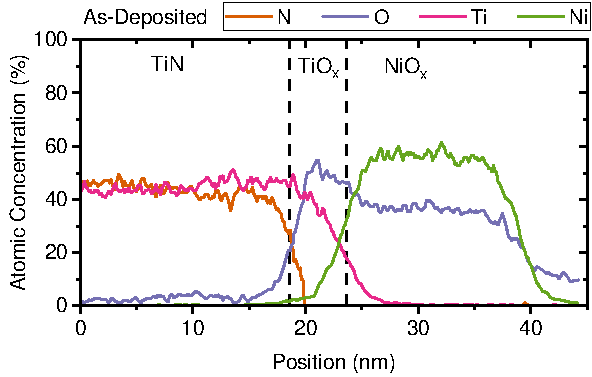
\includegraphics[width=\textwidth]{chapters/material_properties/images/TEM_As_Dep.pdf} % Replace with your image file
        \caption*{(a)}
    \end{subfigure}
    \hfill
    \begin{subfigure}[t]{0.49\textwidth}
        \centering
        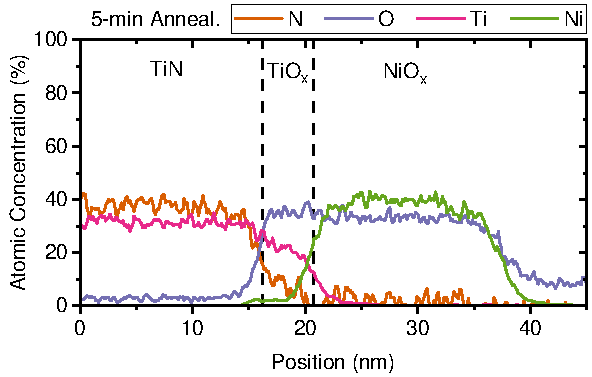
\includegraphics[width=\textwidth]{chapters/material_properties/images/TEM_5_min.pdf} % Replace with your image file
        \caption*{(b)}
    \end{subfigure}


    % Second row
    \begin{subfigure}[t]{0.49\textwidth}
        \centering
        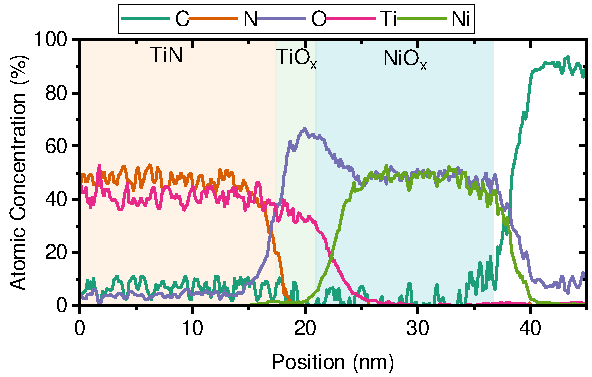
\includegraphics[width=\textwidth]{chapters/material_properties/images/TEM_30_min.pdf} % Replace with your image file
        \caption*{(c)}
    \end{subfigure}
    \hfill
    \begin{subfigure}[t]{0.49\textwidth}
        \centering
        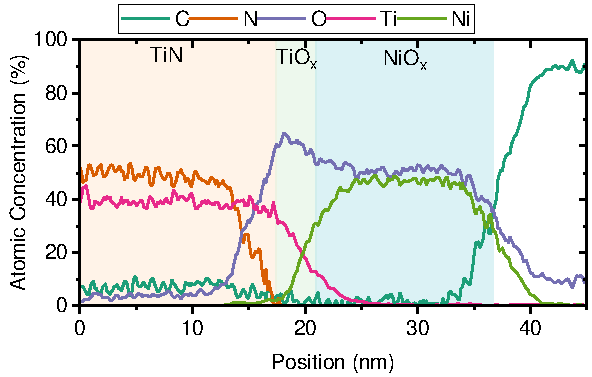
\includegraphics[width=\textwidth]{chapters/material_properties/images/TEM_60_min.pdf} % Replace with your image file
        \caption*{(d)}
    \end{subfigure}
    \caption{TEM of TiN - NiOx interface and emergence of TiOx at the interface.}
    \label{fig:ch2:tem_pix_substrate}
\end{figure}

\section{Conclusions}

Perovskite are known for their defect tolerant structure, this means that variation from the perfect stoichiometry do not have a negative impact on the performance of the device. This has an opposite effect at the same time, that despite pursuing changes in the composition and the fabrication does not translate to a major impact on the the device performance. 



%%%%%%%%%%%%%%%%%%%%%%%%%%%%%%%%%%%%%%%%%%%%%%%%%%
% Keep the following \cleardoublepage at the end of this file, 
% otherwise \includeonly includes empty pages.
\cleardoublepage

